\documentclass{beamer}

\usepackage{beamer_tom}
\usepackage{hyperref}
\graphicspath{{./images/}}

\usepackage{stackengine}
\usepackage{scalerel}
\usepackage{xcolor}
\newcommand\dangersign[1][2ex]{%
  \renewcommand\stacktype{L}%
  \scaleto{\stackon[1.3pt]{\color{red}$\triangle$}{\tiny\bfseries !}}{#1}%
}

\institute{INRIA Saclay}
\author{Thomas Moreau}
\title{
    Sharing Computational Resources:\\
    Some good practices
}

\date{
    May 29, 2018
}

\setbeamertemplate{title page}[frame]
\def\extraLogo{}

\begin{document}

    \begin{frame}
        \titlepage
    %	\biblio{}
    \end{frame}

    \frame{
        \frametitle{Parietal Computational Resources}
        {\large \bf Single Machines:\keypoint{small scale}\\[.5em]}
            \myitem{} drago/2/4 | paradigm/paradox/parametric/parabolic (\emph{CPU})\\
            \myitem{} drago3/5 (\emph{GPU}) \keypoint{(avoid CPU intensive tasks)}\\[.7em]
        {\large \bf Clusters: \keypoint{large scale}\\[.5em]}
            \myitem{} margaret (\emph{SLURM}; $32 \times 40$ CPUs)\\
            \myitem{} tompouce (\emph{SGE}; 288 cores; deprecated)\\[.7em]
        {\large \bf Storage:\\[.5em]}
            \myitem{\texttt{\$HOME}} (\emph{10GB} / user; \code{/home/parietal/\$USER} shared on \code{drago*})\\
            \myitem{dragostore/2} (\emph{130TB}; \code{/storage/store} on \code{drago*} servers)\\[.7em]
        {\large \bf Virtual Machines:\\[.5em]}
            \myitem{} minidrago (\emph{windows}; connection RDP)\\
            \myitem{} Gulliver (\emph{openStack}; see \href{https://gitlab.inria.fr/clusters-saclay/gulliver/blob/master/quickstart.md}{documentation})

    }

    \frame{
        \frametitle{Computation Priority}

        Internally, different processes are managed by the system scheduler:\\[.5em]
        {\centering \large $\Rightarrow$ Who run when?\\[1em]}

        {\bf Rational:} Heavy computation should not block the basic operation!\\[1em]

        Decision are influenced by niceness \code{[-20, 20]}:\\[.5em]
        \myitem{} System process: (Ni<0 : \code{\color{red} Red} in \code{htop})\\
        \myitem{} Base user process: (Ni = 0 : \code{\color{green} Green} in \code{htop})\\
        \myitem{} Nice user process: (Ni > 0 : \code{\color{blue} Blue} in \code{htop})\\[2em]


        {\bf Convention:} Use \code{Ni=5} for computations on Parietal machines.
    }


    \frame{
        \frametitle{Setting niceness}

        Use the \code{nice} command to set the niceness of your process:\\[.5em]
        {\centering \code{nice -5 python myscript.py} \\[1em]}

        More info: \code{man nice}\\[2em]

        {\bf Tips:}\\[.5em]
        \myitem \parbox[t]{.9\textwidth}{
            Set an alias for computation heavy commands \emph{e.g.}\\[.3em]
            \code{alias python="nice -n 5 python"}}\\[1.5em]


        {\bf Extra tip:}
        If you forgot, you can always renice your script:\\[.5em]
        {\centering
            For one script with pid \code{\$PID}:
                \code{renice -n 5 -p \$PID} \\
            For a parallel script with group id \code{\$PGRP}:
                \code{renice -n 5 -g \$PGRP} \\[2em]}
    }


    \frame{
        \frametitle{htop}

        {
        \centering
        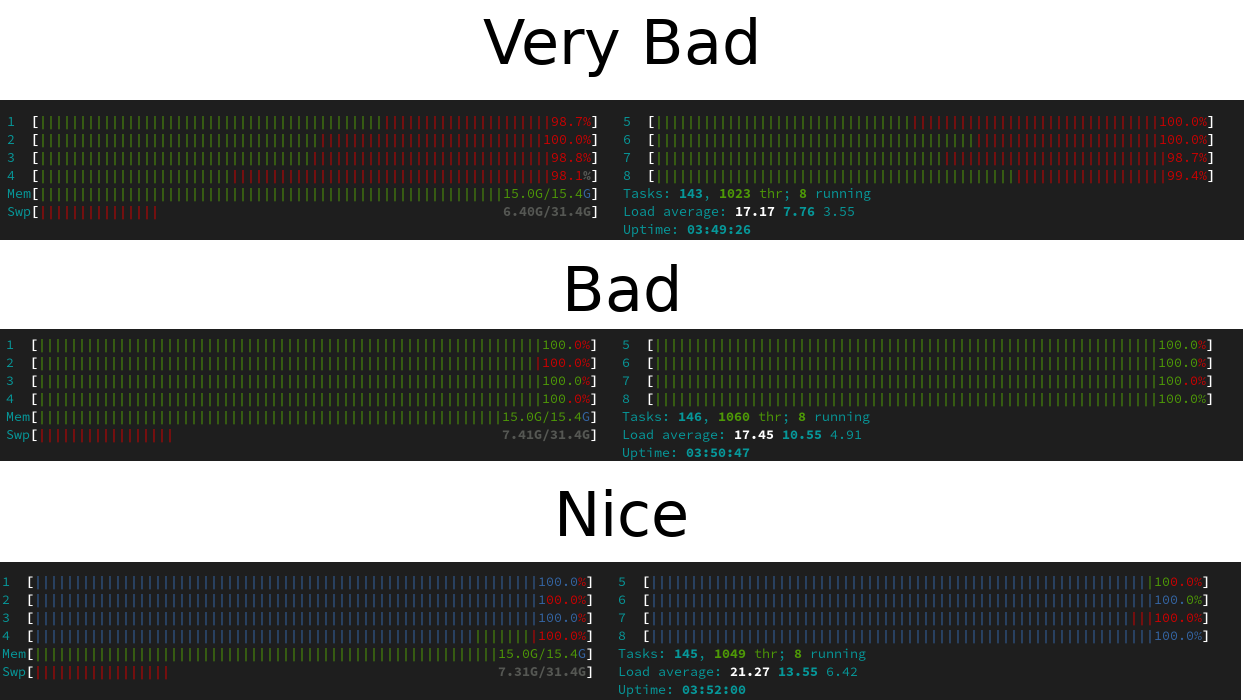
\includegraphics[width=\textwidth]{htop}
        }
    }

    \begin{frame}[t]{Margaret}

        {\bf SLURM: } Intelligent scheduler for a cluster.\\[1em]

        \raisebox{-1ex}{\dangersign[4ex]} \code{\$ ssh margaret} $\Rightarrow$ on the front node, do not run your computation!\\[1em]

        \myitem{} Install your conda in \code{/scratch}; not \code{\$HOME}\\[1.5em]

        {\bf To run your computations}\\[.5em]
        \myitem{} \code{\$ srun -N 1 python script.py} run python script with 1 node.\\[.5em]
        \hskip6ex Use \code{-n 20} to have only 20 CPUs.\\[.5em]
        \myitem{} \code{\$ srun -N 1 -\--pty bash -i} interactive bash on 1 node.\\[2em]



        {\bf Other cmd:}  \code{squeue}, \code{sinfo}, \code{gnodes}, \code{sbatch}, \code{salloc},

    \end{frame}

\end{document}